\subsection{Front-end}
    The front-end application is the control panel of the entire Yako platform. One of the key considerations when designing the application was, for this to be available to be used from any device. The software has been developed with the latest web technologies. It is a multi-platform application, hence, the software can be ran in diverse OS and supports mainstream platforms Microsoft Windows, Linux, Apple macOS, among others. This chapter discusses the process, iterations and changes the project has undergone. From the idea conception through the design process to the technology stack being used.
    
    \subsubsection{Architecture and Technologies}
        As presented in figure \ref{fig:simple_architecture} of the current chapter, the application user interface is built with VueJS \cite{vuejs_what_nodate}, a progressive web framework with the leverage of ElectronJS \cite{openjs_foundation_electron_nodate} which makes it possible to share one code base, build and distribute for different platforms.
        
        ElectronJS embeds Chromium and NodeJS into its binary. While Chromium is an open-source browser project in charge of displaying the content built with VueJS library, NodeJS is the server runtime environment that adds extensive APIs to access the file system and other OS features like networking and I/O. These characteristics are later used in different parts of the application, for instance, when accessing the file system to upload an application or when interacting with the platform API.
        
        \subsubsubsection{Application Architecture}
            The architecture of the front-end application is component-based \cite{dhaduk_component-driven_2021}. As opposed to monoliths, it adopts a modular approach that decomposes front-end UI, taking advantage of benefits like flexibility, responsibilities decoupling, similar to micro-services at the back-end.
        
            \begin{figure}[H]
                \centering
                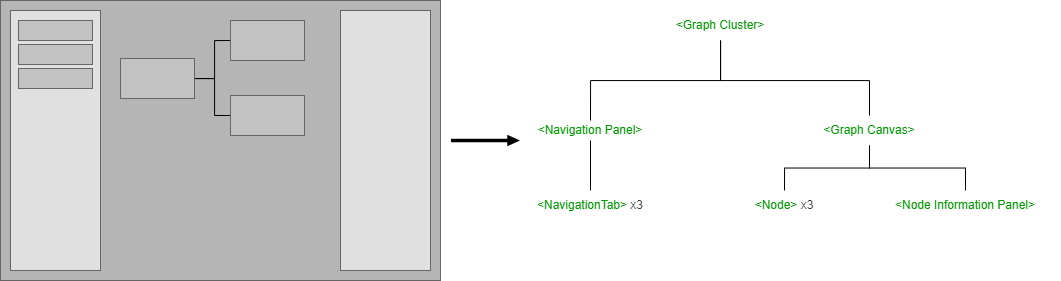
\includegraphics[width=\linewidth]{Frontend/components.png}
                \caption{Component-based UI}
                \label{fig:vue_components}
            \end{figure}
            
            Figure \ref{fig:vue_components} illustrates the Cluster Graph page, one of the views from the YakoUI application. Using VueJS components, enables splitting the UI into independent and reusable pieces. The application is then organized into a tree of nested components.
        
        \subsubsubsection{State handling}
            To handle the UI data changes, VueJS, listens to data change events and re-renders the UI to display that change. The communication between components is through the propagation of properties. which works fine for smaller scale applications. However, due to the natural growth of the software, Vuex \cite{vuejs_what_nodate}, a state management library has been used. The framework is the View component of the Flux pattern \cite{facebook_flux_nodate}.
            
            To modify the values of this global centralized store, an event must be triggered from the view, which would be sent to the dispatcher. The dispatcher then broadcasts the resulting payload which updates the store.
            
            \begin{figure}[H]
                \centering
                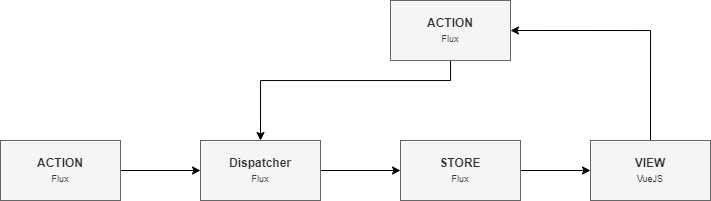
\includegraphics[width=\linewidth]{Frontend/flux.png}
                \caption{Vuex flux pattern}
                \label{fig:flux}
            \end{figure}
            
            At some parts of the project, the Provide / Inject \cite{vuejs_provide_nodate} feature has been used to pass data from the great-grandfather, namely any root component, to the leaf children components as shown in figure \ref{fig:provide_inject}, as opposed to components properties propagation which would lead to a prop-drilling issue.

            \begin{figure}[H]
                \begin{minipage}{0.5\textwidth}
                    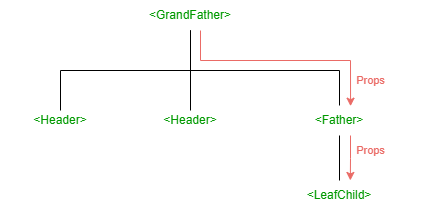
\includegraphics[width=\textwidth]{Images/Frontend/no_provide_inject.png}
                    \subcaption{Prop-drilling effect}
                    \label{code:no_provide_inject}
                \end{minipage}
                \begin{minipage}{0.5\textwidth}
                    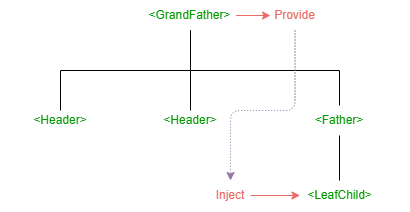
\includegraphics[width=\textwidth]{Images/Frontend/provide_inject.png}
                    \subcaption{Provide - Inject}
                    \label{fig:provide_inject}
                \end{minipage}
                \label{fig:props_propagation}
                \caption{Components properties propagation}
            \end{figure}
        
    
    \subsubsection{Project Structure}
        The project source code structure is divided into 5 big folders:
        
        \begin{itemize}
            \item \textbf{Pages:} Contains the views of the application. For the final software, Upload Application page, Dashboard page and page were developed
            \item \textbf{Components:} Contains all the source code for the developed components for the project
            \item \textbf{Router:} Contains the logic for switching the pages of the application
            \item \textbf{Services:} Contains API endpoints to interact with the Yako platform and other utilities logic used across the software
            \item \textbf{Store:} Logic of Vuex, the global state management
        \end{itemize}

        The following UML diagram shows the relationship of the different components used in the software.
        
        \begin{figure}[H]
            \centering
            \includegraphics[width=0.8\linewidth]{/Frontend/yakoui UML.png}
            \caption{YakoUI project UML}
            \label{fig:yakoui_uml}
        \end{figure}
        
        
    \subsubsection{Project Development}
        Project development sub-section covers the design phase of the application and the stages needed to bring this to life. The first iteration was to design wireframes. After this first iteration, more accurate UI designs were made. Which are the schemes of the look and feel of the final application. The last iteration involved converting the designs to code.
        
        \subsubsubsection{Stage 1: Wireframing}
            At the early stages of the project, mid-fidelity wireframes were designed to accurately represent the layout and clearly portray the information architecture of what would become the panel of the platform.
            In the following designs, user flow and functionalities are outlined.
    
            \subsubsubsubsection{Cluster graph wireframe}
                The cluster graph wireframe consisted in designing a view tab where the system administrator could view all the nodes (YakoMasters and YakoAgents) in the system, and how these are interconnected. The right side panel space is allocated to show additional information about the selected device.
                
                \begin{figure}[H]
                    \centering
                    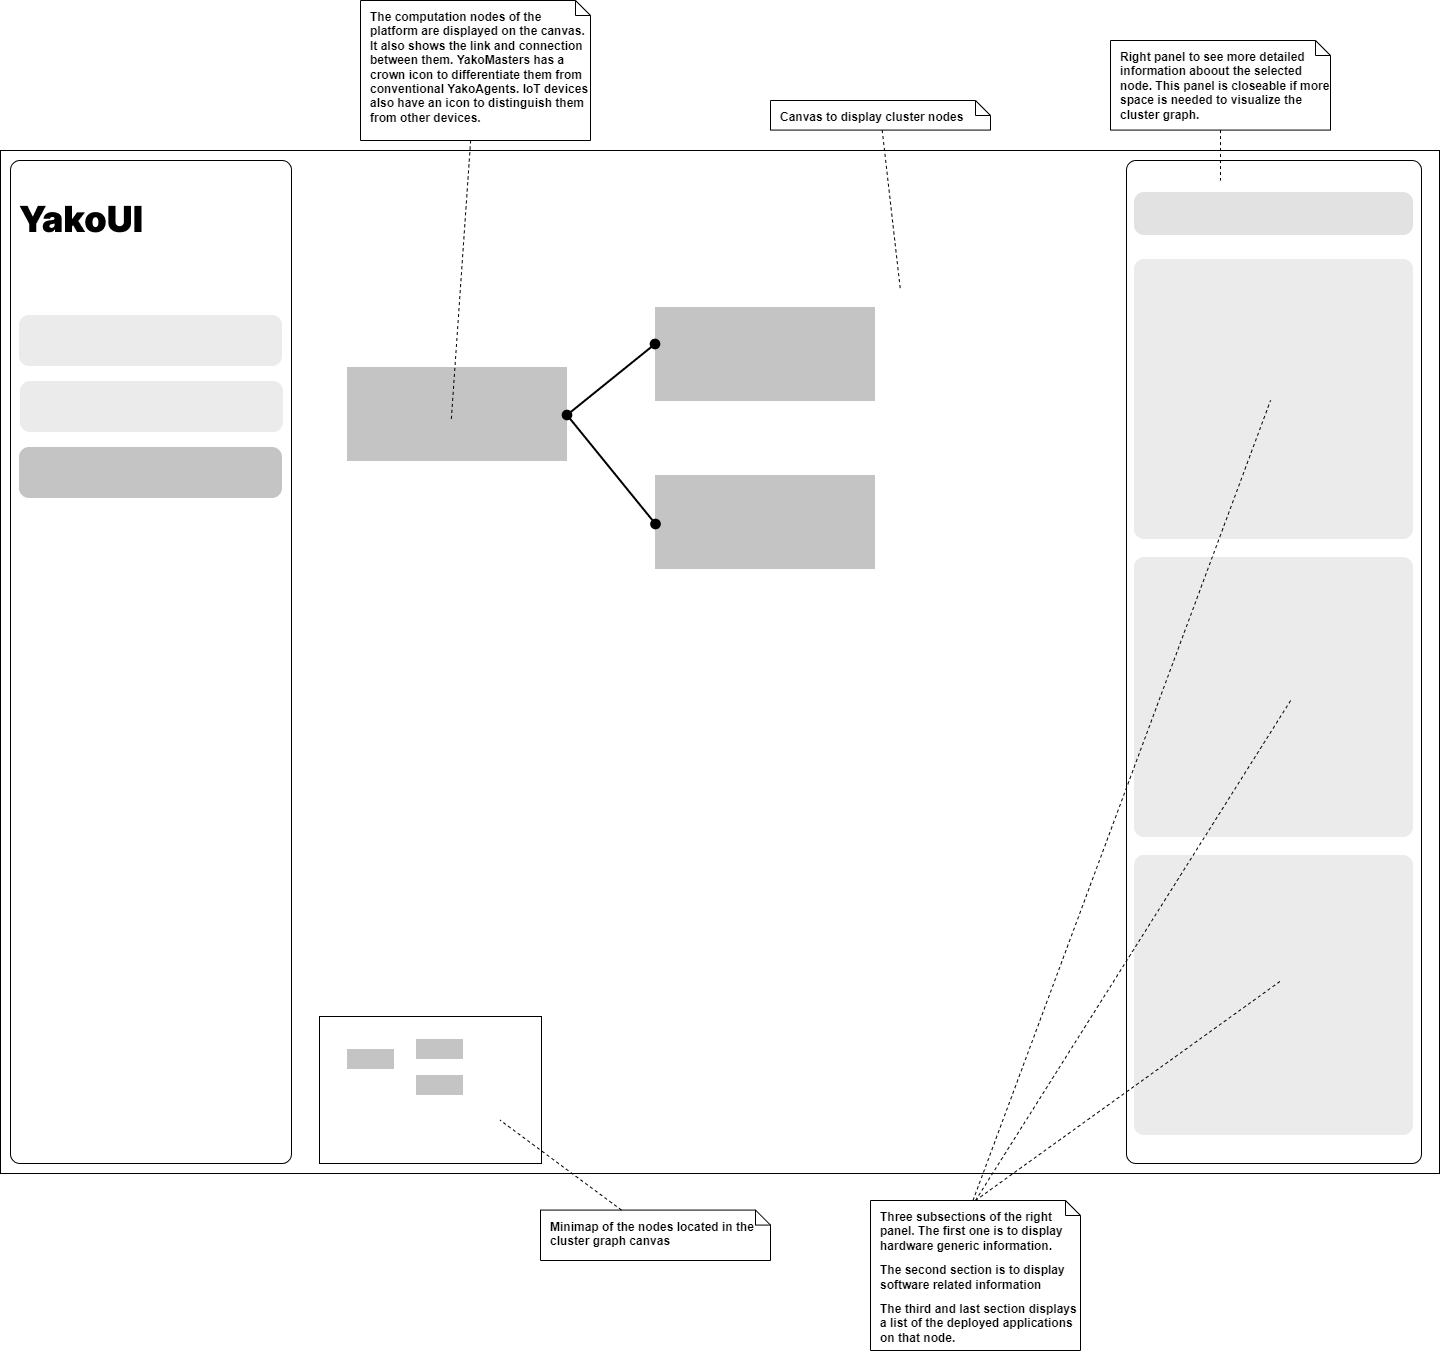
\includegraphics[width=0.8\linewidth]{/Frontend/YakoUI cluster graph wireframe.png}
                    \caption{YakoUI cluster graph wireframe}
                    \label{fig:cluster_wireframe}
                \end{figure}
                
            \subsubsubsubsection{Dashboard wireframe}
                This view tab is where all the information is gathered. The same nodes are shown in the left side of the page. On the top right side, a list of the top YakoAgent where the previously uploaded application could be uploaded are shown in descent order.
                The down right corner is reserved to display a list of the previously deployed application.
                
                \begin{figure}[H]
                    \centering
                    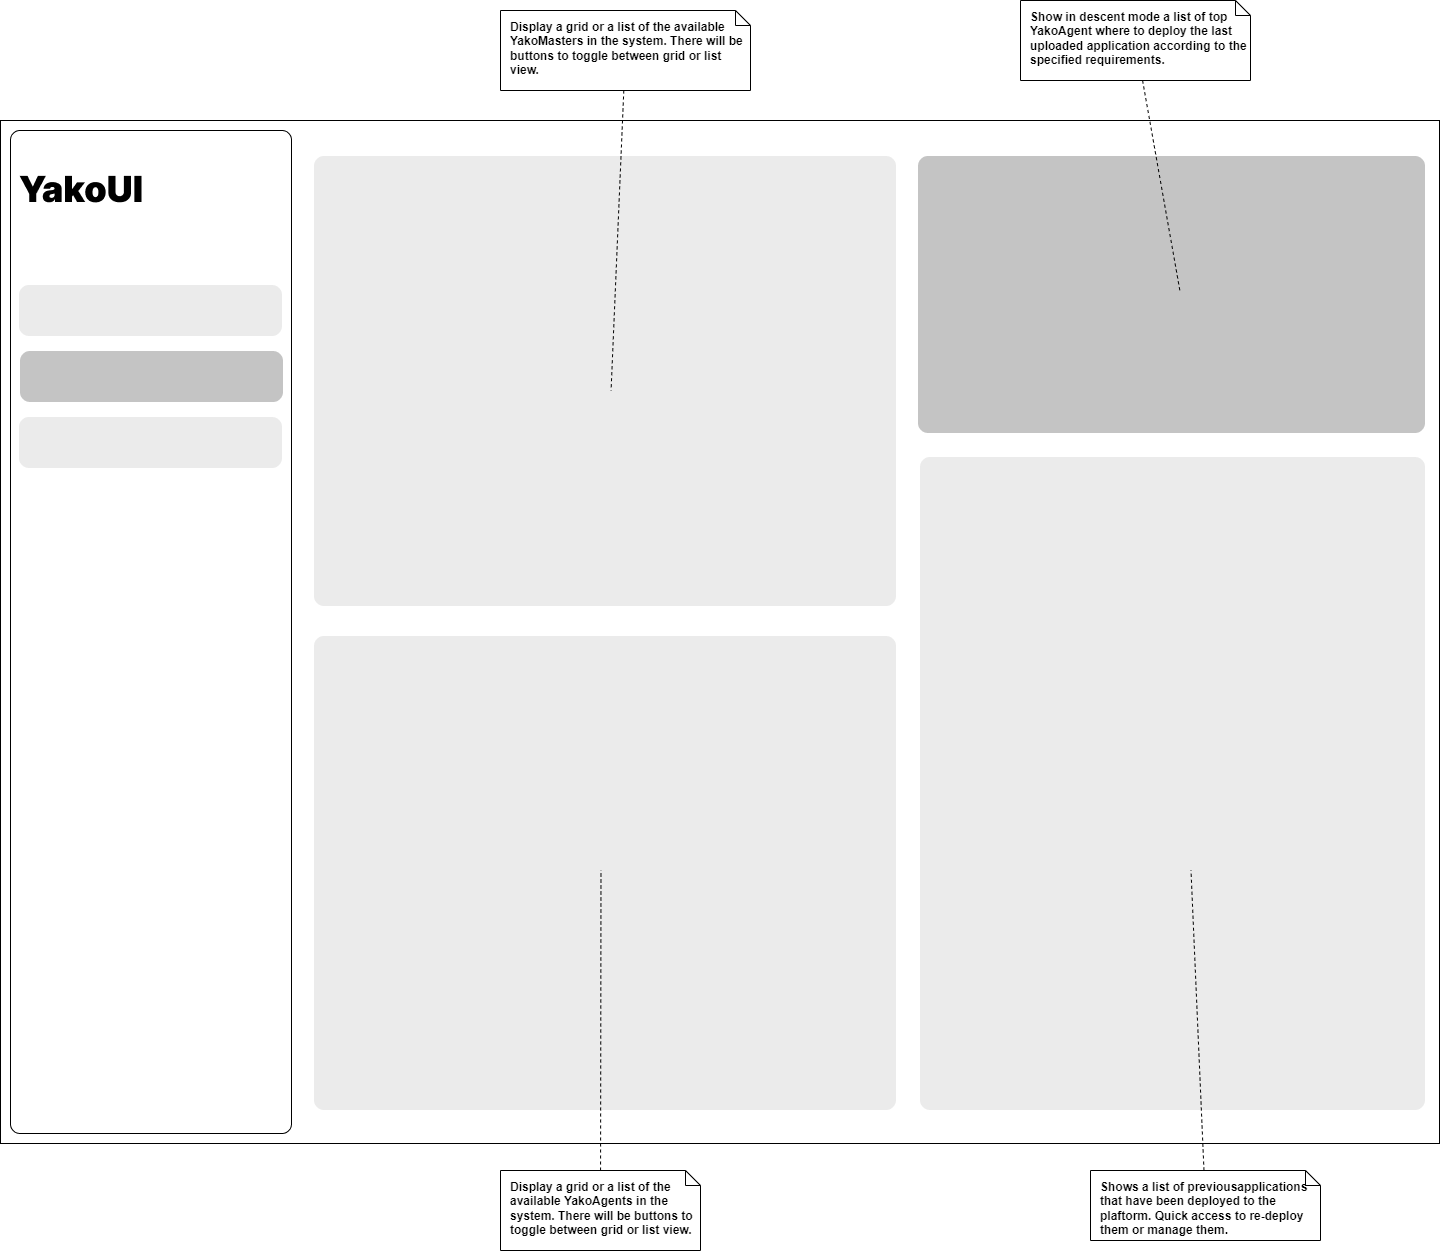
\includegraphics[width=0.8\linewidth]{/Frontend/YakoUI Dashboard wireframe.png}
                    \caption{YakoUI dashboard wireframe}
                    \label{fig:dashboard_wireframe}
                \end{figure}
                
            \subsubsubsubsection{Upload and Deploy application wireframe}
                This view tab is the entry point of the platform. It will be shown on application start up, a drag and drop area is shown in the center where the system administrator could select the application to be deployed in the system.
                
                \begin{figure}[H]
                    \centering
                    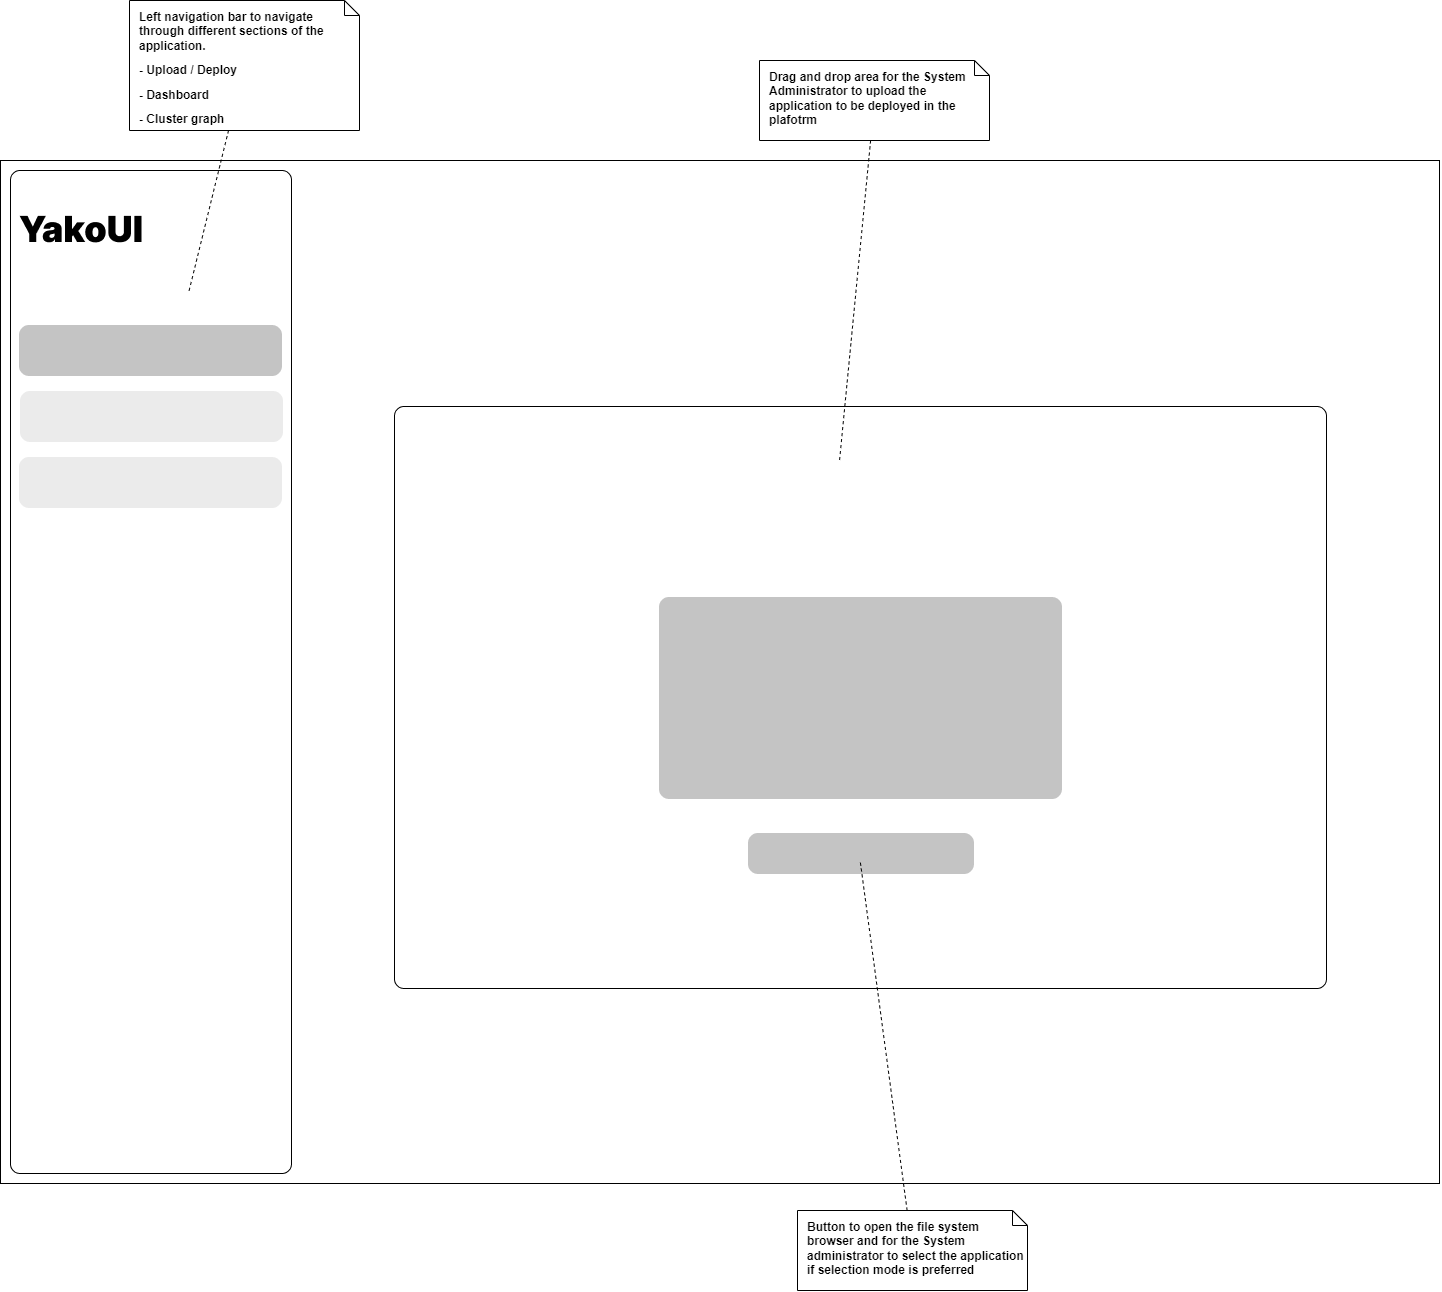
\includegraphics[width=0.8\linewidth]{/Frontend/YakoUI deploy app wireframe.png}
                    \caption{YakoUI deploy app wireframe}
                    \label{fig:deploy_wireframe}
                \end{figure}
        
        \subsubsubsection{Stage 2: UI prototyping}
            In this second stage, all the previous low-fidelity wireframes were converted into UI prototypes. These includes more details on the sections. In this step a design system was defined.
            
            \subsubsubsubsection{Dashboard User Interface}
                The dashboard page provides a visual display of the platform. The view is divided horizontally in two sections, on the left side there are two subsections where the information about all the agents including the YakoMasters are displayed. For usability purpose, located on the top right corner of these sections two views styles buttons, grid and list, have been provided. Toggling between them will change the displaying format.
                
                On the other half of this page, two other sections are reserved to display Top Nodes and the list of uploaded Applications. The node cards should display the agent identifier and the resources that comply with the requested system resources are highlighted in green, while those that do not fulfil are marked in red.
                
                The enumerations of the Applications section are presented as a list of application cards. These cards show the application name on the left side, and buttons to interact with these are situated on the other side.
                \begin{figure}[H]
                    \centering
                    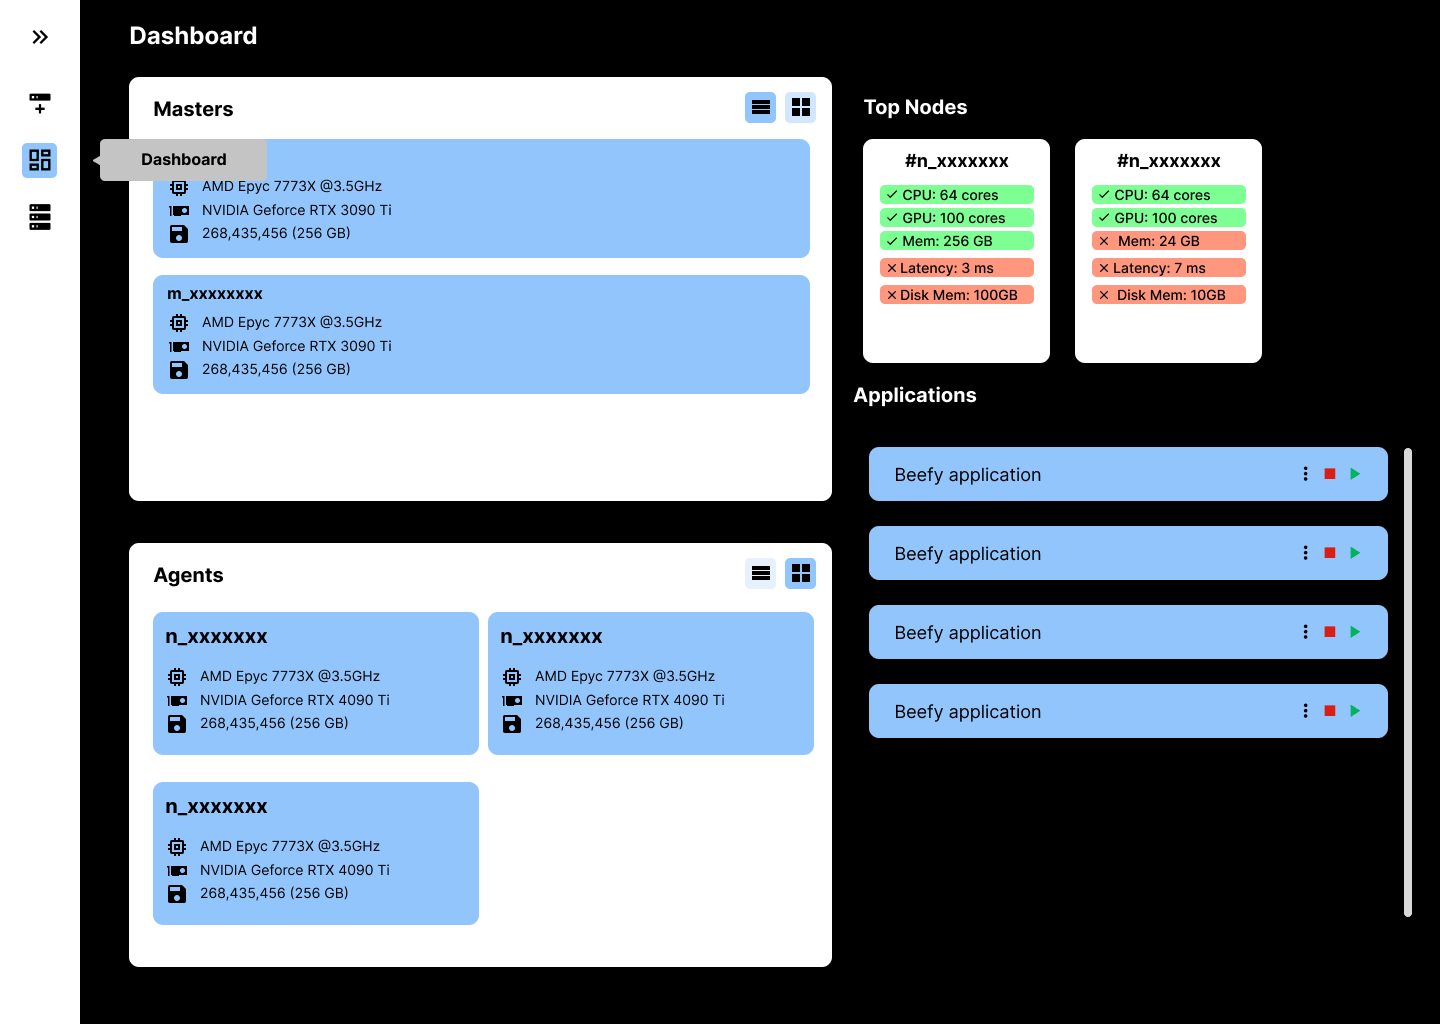
\includegraphics[width=\linewidth]{Images/Frontend/UI/YakoUI Dashboard UI.png}
                    \caption{YakoUI dashboard UI}
                    \label{fig:dashboard_ui}
                \end{figure}
            
            \subsubsubsubsection{Cluster graph User Interface}
                The Cluster Graph page shows available nodes in a graphical mode. An extended version of the data is situated in the right side. It can be displayed at user's convenience by clicking on any of the nodes. This panel is divided into 4 main sections, General Information, System Information, Network Information and Deployed Applications lists shows the active running applications on that node.
                
                An even more detailed version of the previously expanded right panel, figure \ref{fig:expanded_info_panel_ui},  can be shown by clicking the left chevron tab situated in the left center part. On click it will enlarge the floating window showing the same amount of previous information with the addition of several graphs and telemetry in graphical mode.
            
                \begin{figure}[H]
                    \centering
                    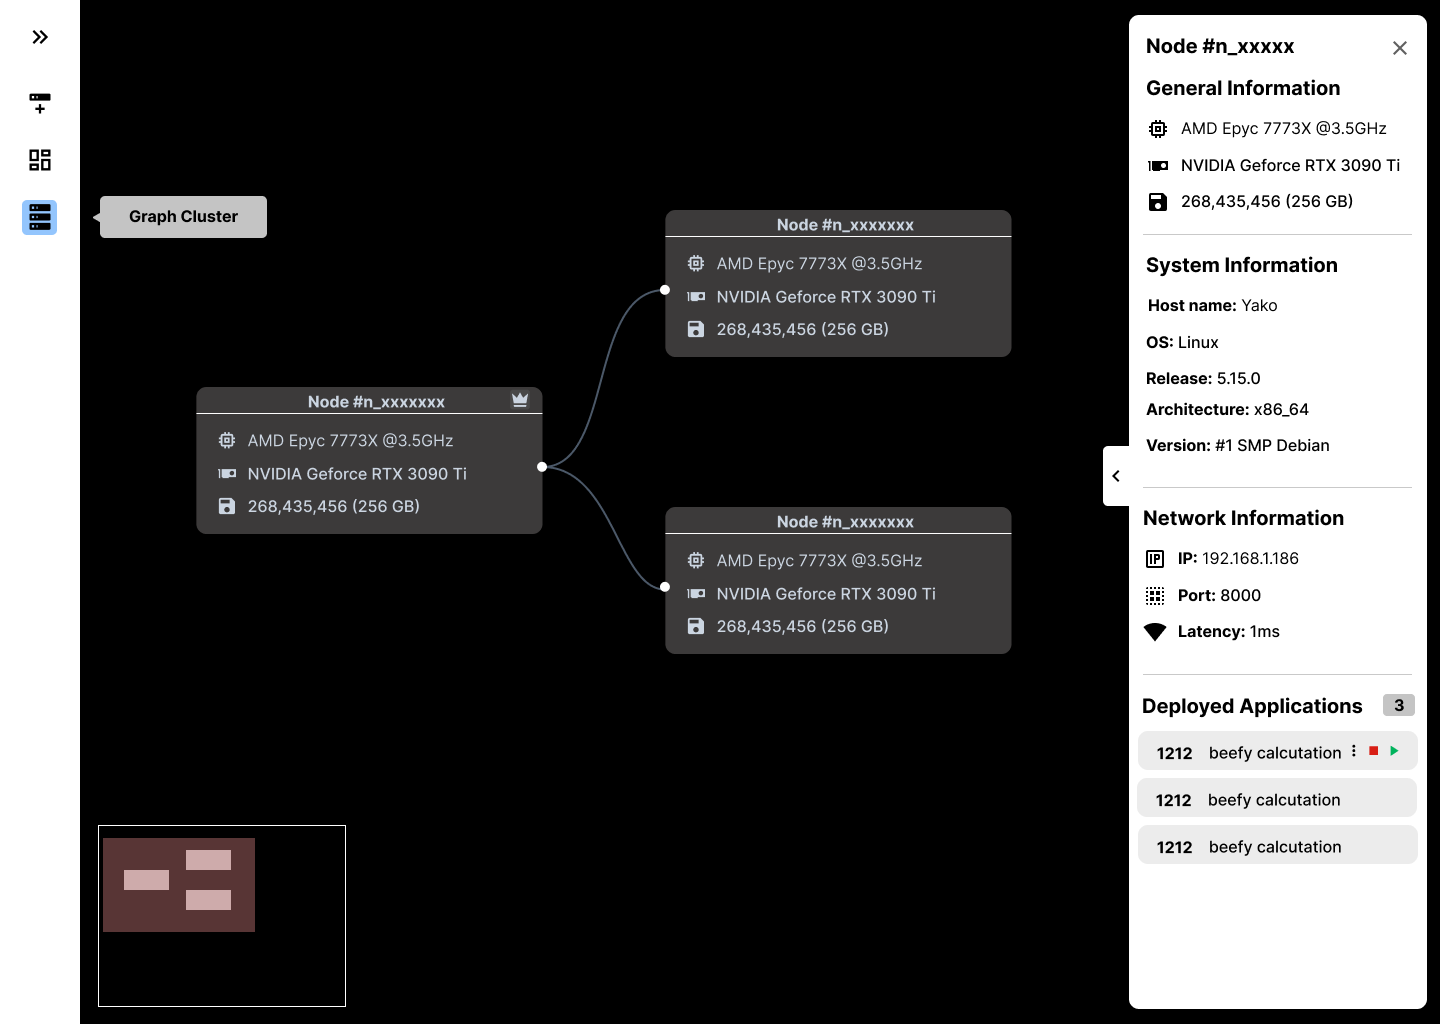
\includegraphics[width=0.85\linewidth]{Images/Frontend/UI/YakoUI Graph Cluster UI.png}
                    \caption{YakoUI Cluster Graph UI}
                    \label{fig:cluster_graph_ui}
                \end{figure}
                
                This view, figure \ref{fig:expanded_info_panel_ui},  was not developed for the delivered v1 software, due to time constraints and the prioritization of other major features.
                
                \begin{figure}[H]
                    \centering
                    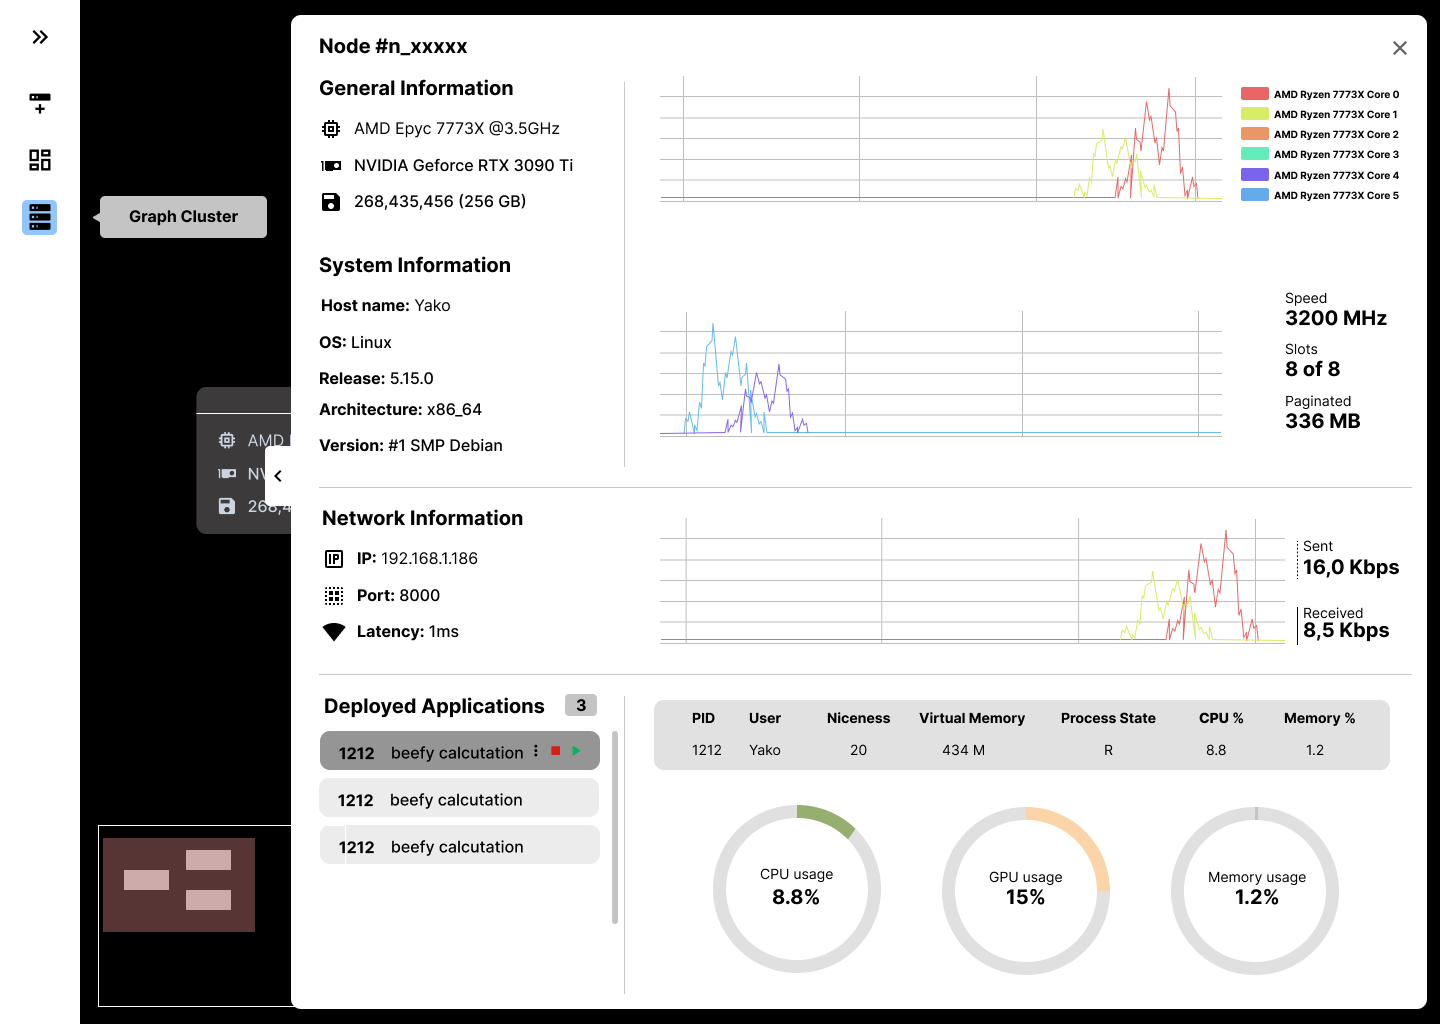
\includegraphics[width=0.85\linewidth]{Images/Frontend/UI/YakoUI Expanded YakoAgent Information Panel UI.png}
                    \caption{YakoUI Expanded YakoAgent Information Panel UI}
                    \label{fig:expanded_info_panel_ui}
                \end{figure}
            
            \subsubsubsubsection{Upload and Deploy application User Interface}
                This is the first page that will be presented to the user on application start up. This view consists of a region where the system administrator can drag and drop the application to be deployed in the cluster. If manual selection is preferred, a "Select file" button is made available.
                
                \begin{figure}[H]
                    \centering
                    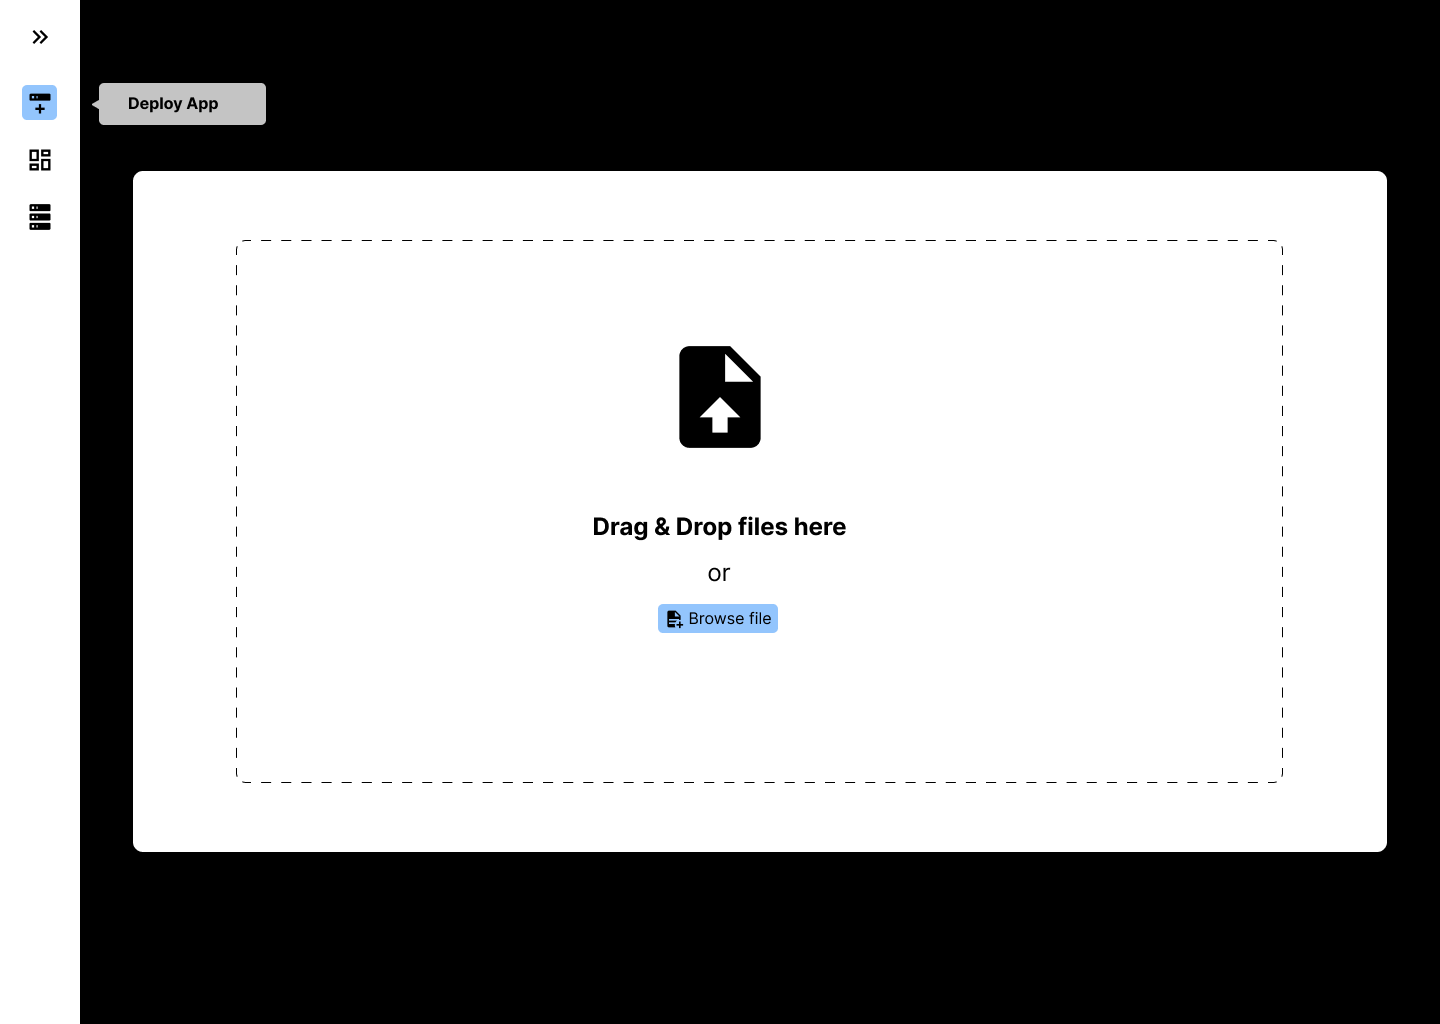
\includegraphics[width=0.7\linewidth]{Images/Frontend/UI/YakoUI Upload Application UI.png}
                    \caption{YakoUI Deploy Application UI}
                    \label{fig:deploy_app_ui}
                \end{figure}
            
                Once the application has been selected, a pop-up form will appear, figure \ref{fig:upload_form}.
                
                \begin{figure}[H]
                \centering
                    \begin{subfigure}{0.45\textwidth}
                        \centering
                        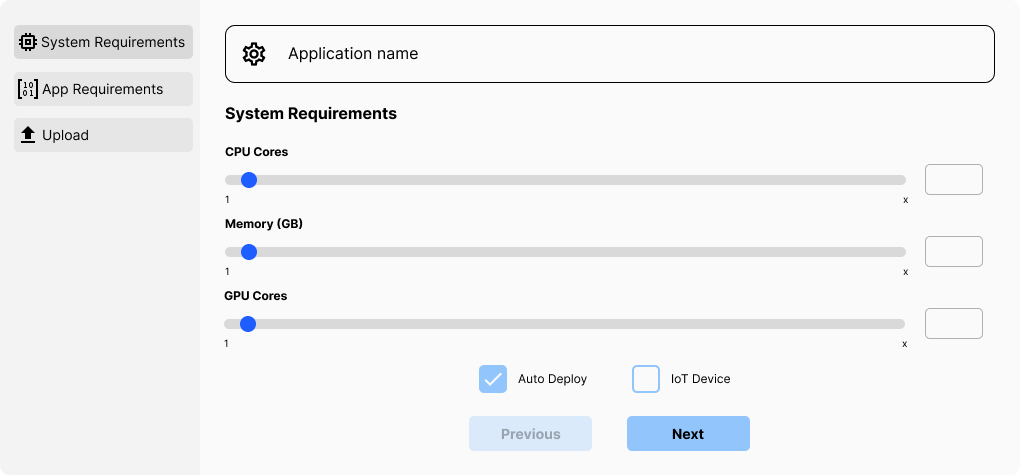
\includegraphics[width=\textwidth]{Images/Frontend/UI/YakoUI Form 1.png}
                        \subcaption{System Requirements form}
                        \label{fig:form_1}
                    \end{subfigure}
                    \begin{subfigure}{0.45\textwidth}
                        \centering
                        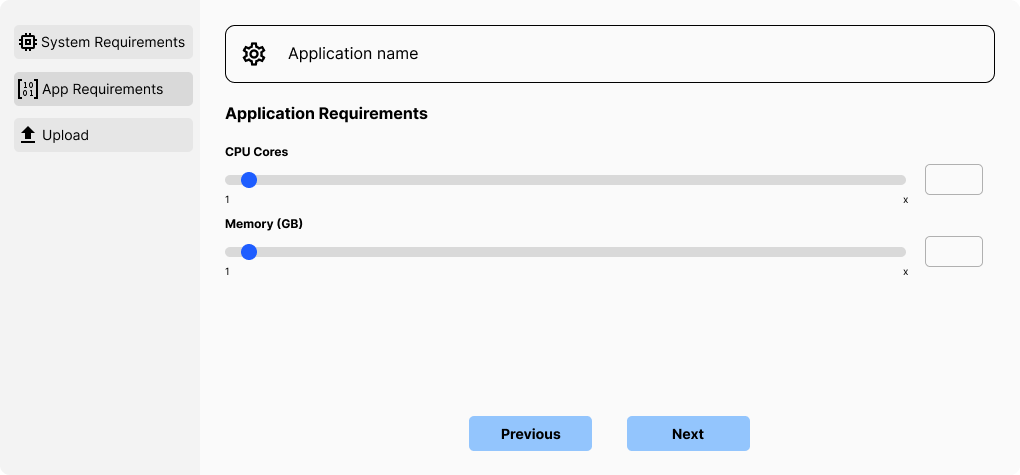
\includegraphics[width=\textwidth]{Images/Frontend/UI/YakoUI Form 2.png}
                        \subcaption{Application Requirements form}
                        \label{fig:form_2}
                    \end{subfigure}
                    \vskip\baselineskip
                    \begin{subfigure}{\textwidth}
                        \centering
                        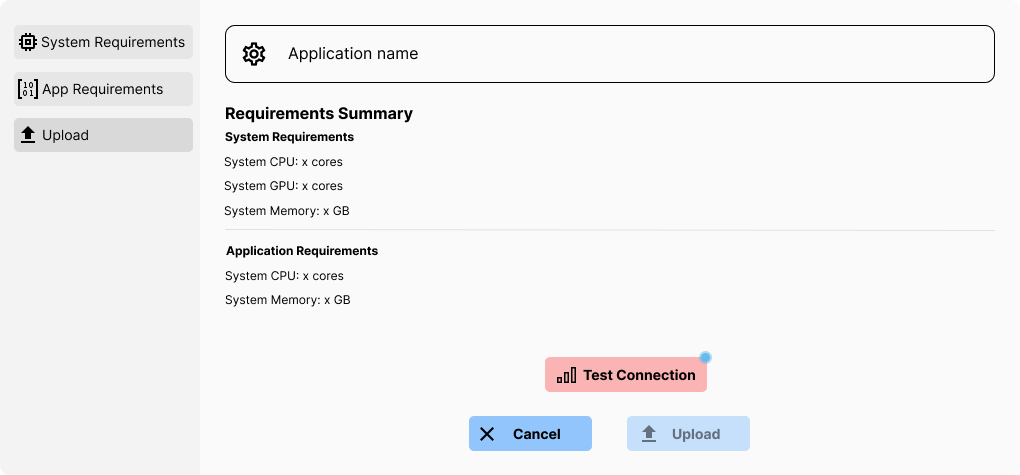
\includegraphics[width=0.45\textwidth]{Images/Frontend/UI/YakoUI Form 3.png}
                        \subcaption{Summary form tab}
                        \label{fig:form_3}
                    \end{subfigure}
                    \caption{Upload application form}
                    \label{fig:upload_form}
                \end{figure}
                
                This window contains 3 tabs. The first asks the user to select all the preferred specifications of the system where the binary will be ran. These system requirements specifications will be collected to find the most suitable node of the cluster.
                The following tab collects resources for the virtualization of the application (The back-end logic for this feature could not been developed for release v1).
                The last tab summarizes all the selected properties. A connection test must be fired before being able to upload and deploy the application.